\section{Beautiful Colours}

\rfig{fig:colours} displays a beautiful set of colours, some of them are warm colours and others are cold colours. They are all very beautiful, we suggest to the reader to have a look at them.
\begin{figure}[h!]
    \centering
    \begin{subfigure}[b]{0.3\textwidth}
        
\includegraphics[width=\textwidth]{red.png}
        \caption{Red}
        \label{fig:red}
    \end{subfigure}
    \quad
    \begin{subfigure}[b]{0.3\textwidth}
        
\includegraphics[width=\textwidth]{yellow.png}
        \caption{Yellow}
        \label{fig:yellow}
    \end{subfigure}
    \quad
    \begin{subfigure}[b]{0.3\textwidth}
        
\includegraphics[width=\textwidth]{blue.png}
        \caption{Blue}
        \label{fig:blue}
    \end{subfigure}
    \\
    \begin{subfigure}[b]{0.3\textwidth}
        
\includegraphics[width=\textwidth]{orange.png}
        \caption{Orange}
        \label{fig:orange}
    \end{subfigure}
    \quad
    \begin{subfigure}[b]{0.3\textwidth}
        
\includegraphics[width=\textwidth]{green.png}
        \caption{Green}
        \label{fig:green}
    \end{subfigure}
    \caption{Very beautiful colours}
    \label{fig:colours}
\end{figure}

The three warm colours in \rfig{fig:colours} are red (\rfig{fig:red}), yellow (\rfig{fig:yellow}) and orange (\rfig{fig:orange}). The two cold colours in \rfig{fig:colours} are blue (\rfig{fig:blue}) and green (\rfig{fig:green}).

\clearpage

\section{Canny edge detector}

Colours are overrated, true information is gathered by living on the edge.

\begin{figure}[h!]
% \begin{figure}[H]
    \centering
    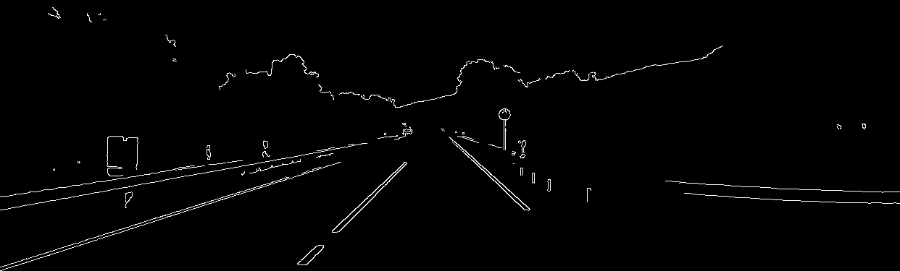
\includegraphics[width=0.9\textwidth]{road2_900Canny.png}
    \caption{Edges detected with Canny}
    \label{fig:road2_canny}
\end{figure}


